\section{Helióstato}
\label{sec:helio}

\begin{problem}
  Realizar el trazado de rayos de un helióstato y un receptor colocado en lo alto de una torre, ver Figura~\ref{fig:helio}. Consideré que el helióstato tiene unas dimensiones de 1$\times$1~m, y se encuentra a 50~m de la torre, hacia el norte. El receptor esta a una altura de 32~m. Considere que el vector solar es igual a $\hat s = (0, 0, 1)$.
\end{problem}

\begin{figure}[ht]
  \centering
  \includegraphics[width=1.0\textwidth]{figures/helio}
  \caption{\label{fig:helio} Heliostato}
\end{figure}


\TheSolution Sabemos que por la ley de reflección podemos calcular la dirección de la normal $\hat n$ del helióstato con la ecuación~\ref{eq:nst}, de donde conocemos $\hat s$ y el vector de reflexión es $\vec R = T - H$ y su valor unitario es de $\hat r = (0.00, -0.8422, 0.5390)$. Por lo que el valor de $\hat n = (0.00, -0.480, 0.877)$.

\begin{equation}
  \label{eq:nst}
  \hat n = \dfrac{\hat s + \hat r}{\| \hat s + \hat r \|}
\end{equation}

El valor del \emph{aimpoint} $\vec A = \vec R_F + \hat n$, donde $\\vec R_F$ es un vector que va del origen a la posición del helióstato, en este caso $\vec R_F = (0, 50, 0)$, y $\vec A = (0, 49.52, 0.877)$.

\ASolution:

Considerese las propiedades ópticas de la Tabla~\ref{tab:opticaHelio} para el helióstato.

\begin{table}[h]
  \centering
  \begin{tabular}[h]{ccccc}
    \toprule
    Reflectivity & Transmissivity & Slope error & Specularity error & Error type\\
    \midrule
    0.95         & 0.0001         & 2.500      & 0.2000            & Gaussian\\
    \bottomrule
  \end{tabular}
  \caption{\label{tab:opticaHelio} Propiedades ópticas}
\end{table}

Nuevamente se requieren dos etapas, una para el helióstato y otra para el receptor. La posición del helióstato es $H = (0, 50, 0)$, y su \emph{aimpoint} es el calculado. El Helióstato tiene una apertura de 1$\times$1~m y en este caso se trata de una superficie plana. La Tabla~\ref{tab:etapaHelioC} indica los parámetros indicados.

\begin{table}[h]
  \centering
  \scriptsize
  \begin{tabular}[h]{lllllllll}
    \toprule
    X-C & Y-C & Z-C & X-AimP & Y-AimP & Z-AimP & Z-Rot & Aperture & Surface\\
    \midrule
    0 & 50 & 0 & 49.52 & 0.877 & 0 & 0 & r-1,1,0,0,0,0,0,0 & p-0,0,0,0,0,0,0,0\\
    \bottomrule
  \end{tabular}
  \caption{\label{tab:etapaHelioC} Etapa del concentrador.}
\end{table}

El receptor, en este caso, se trata de una superficie plana orientada hacia el norte. Dado que no indican el tamaño utilizaremos un receptor de 3$\times$3~m, como lo indica la Tabla~\ref{tab:etapaHelioR}.

\begin{table}[h]
  \centering
  \scriptsize
  \begin{tabular}[h]{lllllllll}
    \toprule
    X-C & Y-C & Z-C & X-AimP & Y-AimP & Z-AimP & Z-Rot & Aperture & Surface\\
    \midrule
    0 & 0 & 32 & 0 & 1 & 32 & 0 & r-3,3,0,0,0,0,0,0 & f-0,0,0,0,0,0,0,0\\
    \bottomrule
  \end{tabular}
  \caption{\label{tab:etapaHelioR} Etapa del receptor }
\end{table}

Posteriormente se realiza una simulación considerando a millón de rayos. La Figura~\ref{fig:rayHelio} muestra la simulación.

\begin{figure}[ht]
  \centering
  \subfigure[]{
    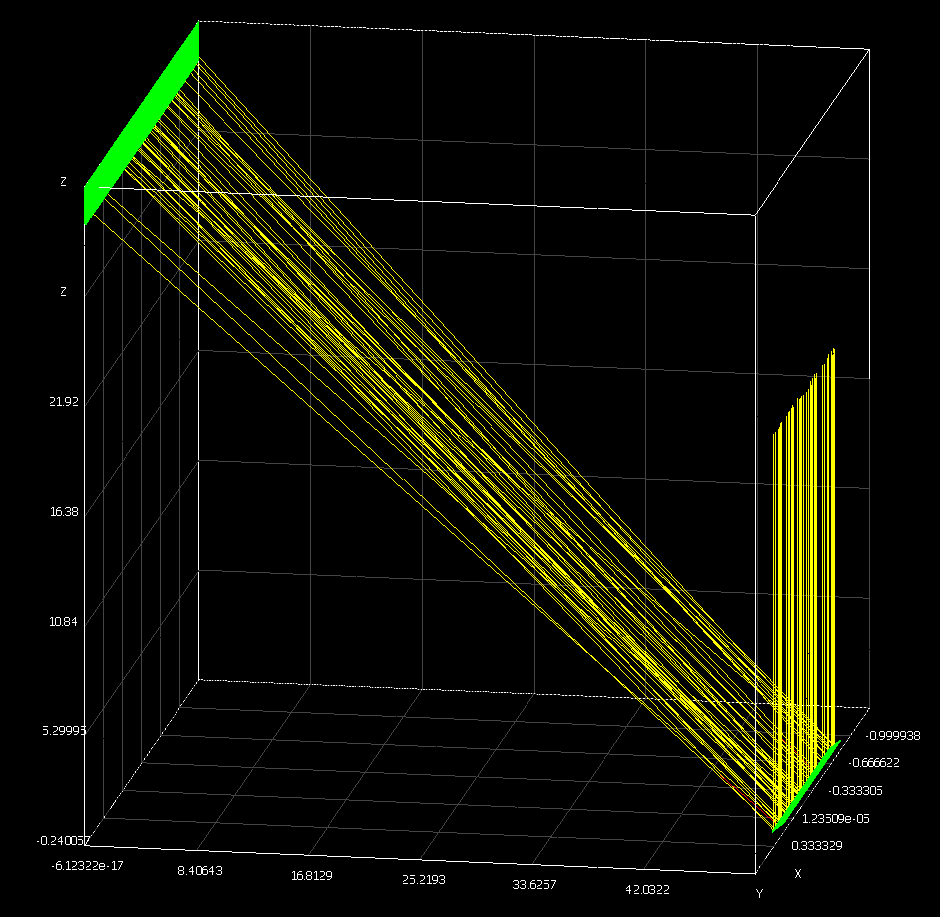
\includegraphics[width=0.33\textwidth]{figures/rayHelio}}
  \subfigure[]{
    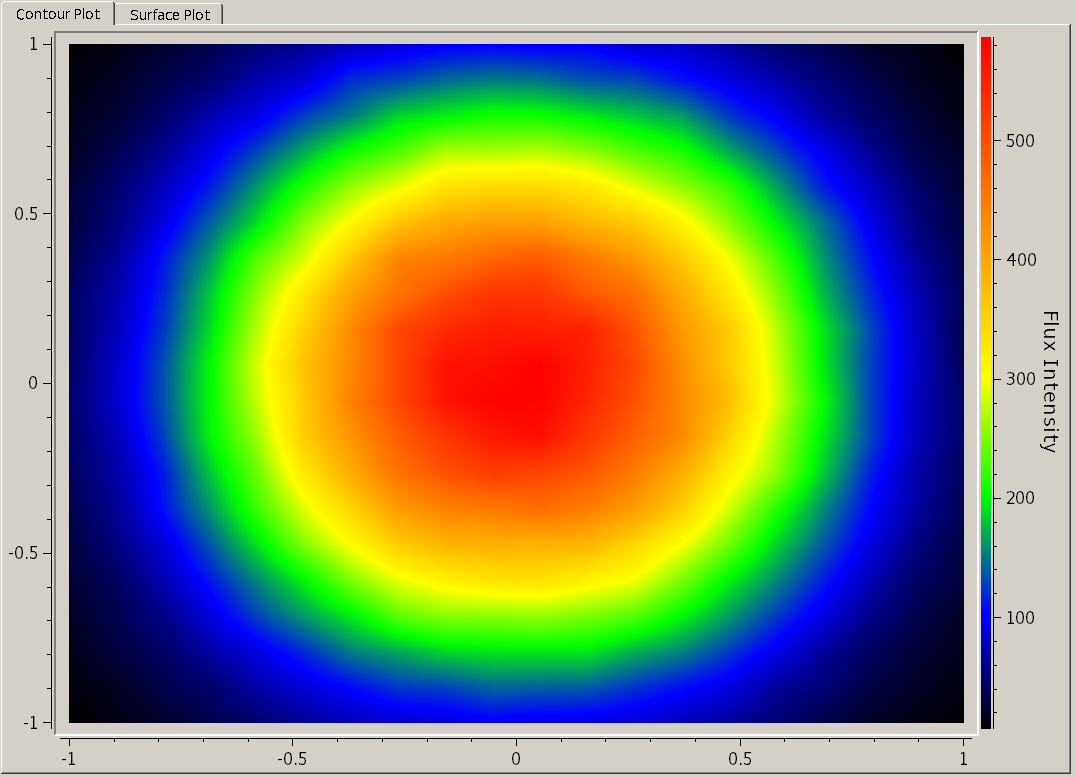
\includegraphics[width=0.45\textwidth]{figures/fluxHelio}}
  \caption{\label{fig:rayHelio} Simulación de trazado de rayos de un helióstato.}
\end{figure}



%%% Local Variables: ***
%%% mode: latex ***
%%% TeX-master: "taller.tex" ***
%%% End: ***
